\section{The data foundation}
\label{sec:data}

\subsection{The FACE cohorts and the baseline visit}
FACE-ATLAS is built on the harmonized baseline (visit \code{V0}) of three FACE expert-centre cohorts. After
harmonization the modelling sample is
\[
N = 9{,}013 \;=\; \underbrace{6{,}252}_{\text{BP}} \;+\; \underbrace{2{,}209}_{\text{SZ}} \;+\; \underbrace{552}_{\text{DR}} ,
\]
fit on the \emph{full} sample with no completeness selection (Chapter~\ref{sec:estimation} explains why this is
a stated acceptance criterion rather than a convenience). The cohort imbalance --- BP is roughly $11\times$ DR
--- is handled by testing measurement invariance and by an optional inverse-frequency-weighted sensitivity arm,
never by discarding data.

\begin{table}[h]\centering\small\sffamily
\caption{Composition of the harmonized V0 modelling sample.}
\label{tab:cohorts}
\begin{tabular}{L{4.0cm} R{2.2cm} R{2.6cm} L{4.6cm}}
\toprule
\hdr{cohort} & \hdr{$N$} & \hdr{share} & \hdr{role}\\
\midrule
\rowcolor{facebg} Bipolar disorder (BP) & 6{,}252 & 69.4\% & entry metadata / validation label\\
Schizophrenia (SZ) & 2{,}209 & 24.5\% & entry metadata / validation label\\
\rowcolor{facebg} Depression (DR) & 552 & 6.1\% & entry metadata / validation label\\
\midrule
\textbf{Total} & \textbf{9{,}013} & 100\% & one global factor structure\\
\bottomrule
\end{tabular}
\end{table}

\subsection{The harmonization dictionary}
A single curated dictionary (\file{data/face-common-vars.xlsx}; 225 rows, 201 usable) is the contract between
the raw cohorts and the model. One row per harmonized variable records: the human label and clinical rationale;
the per-cohort source column (\code{BP}/\code{SZ}/\code{DR}, blank where absent); the target dtype and value
set; per-variable \emph{sanity bounds}; a \emph{readiness} tier (READY for 3-cohort, PARTIAL for 2-cohort, NOT
USABLE excluded); and the canonical harmonized name --- the modelled feature. The data layer loads this
contract; nothing is hand-merged.

The harmonization problem is real: the three cohorts often encode the same variable differently --- BP/SZ store
French text labels where DR stores integer codes; the same column mixes units (milliseconds and seconds for ECG
intervals; g/L and g/dL for haemoglobin concentration); sentinel and ceiling tokens (\code{>10}) contaminate
counts. Each such variable has a registered transformer that reconciles the encodings and records its rule and
provenance.

\subsection{The pipeline: harmonize, bound, decode --- never impute}
The data layer (\file{src/face/data/}) exposes three composable entry points used by the build script. The flow
is shown in Figure~\ref{fig:dataflow}.

\begin{figure}[h]\centering
\resizebox{\linewidth}{!}{%
\begin{tikzpicture}[>={Stealth[length=2.6mm]},node distance=6mm,
   stg/.style={draw=faceaccent,line width=0.7pt,rounded corners=2.5pt,fill=white,
     minimum height=15mm,text width=26mm,align=center,font=\sffamily\footnotesize,inner sep=3pt},
   raw/.style={draw=facemute,line width=0.7pt,rounded corners=2.5pt,fill=facebg,
     minimum height=15mm,text width=22mm,align=center,font=\sffamily\footnotesize,inner sep=3pt},
   outb/.style={draw=facekr,line width=0.9pt,rounded corners=2.5pt,fill=facekr!8,
     minimum height=15mm,text width=24mm,align=center,font=\sffamily\footnotesize,inner sep=3pt}]
  \node[raw] (csv) {\bfseries 3 raw CSVs\\[2pt]\scriptsize BP\,/\,SZ\,/\,DR\\\scriptsize (confidential)};
  \node[stg,right=of csv] (map) {\bfseries dictionary\\\bfseries map\\[2pt]\scriptsize source col $\to$\\\scriptsize canonical name};
  \node[stg,right=of map] (rule) {\bfseries harmonize\\[2pt]\scriptsize text$\to$code,\\\scriptsize unit \& sentinel\\\scriptsize fixes};
  \node[stg,right=of rule] (san) {\bfseries sanity\\\bfseries bounds\\[2pt]\scriptsize out-of-range\\\scriptsize $\to$ NaN};
  \node[stg,right=of san] (skip) {\bfseries skip-logic\\\bfseries decode\\[2pt]\scriptsize gate=No\\\scriptsize $\to$ structural 0};
  \node[outb,right=of skip] (X) {\bfseries harmonized\\$X$\\[2pt]\scriptsize patient $\times$ var,\\\scriptsize NaN = missing};
  \draw[->,faceaccent,line width=0.8pt] (csv)--(map);
  \draw[->,faceaccent,line width=0.8pt] (map)--(rule);
  \draw[->,faceaccent,line width=0.8pt] (rule)--(san);
  \draw[->,faceaccent,line width=0.8pt] (san)--(skip);
  \draw[->,faceaccent,line width=0.8pt] (skip)--(X);
\end{tikzpicture}}
\caption{The no-imputation data pipeline. \code{build_unified_dataframe} reads each per-cohort source column,
applies the harmonization rule and the sanity bounds, and stacks the cohorts; \code{to_harmonized_dataset}
restricts to the baseline visit and applies skip-logic structural-zero decoding. Missing cells remain
\code{NaN} at every stage.}
\label{fig:dataflow}
\end{figure}

\paragraph{Sanity bounds.} Each variable carries plausibility bounds tuned to catch gross scale/unit errors
(a glucose of 488 from a mg/dL slip), \emph{not} to trim genuine clinical extremes. Out-of-range cells are set
to \code{NaN} --- never winsorized to the boundary, never filled. Formally, with bounds $[\ell_j,h_j]$,
\[
X_{ij} \leftarrow \mathrm{NaN}\quad\text{iff}\quad X_{ij}<\ell_j \;\lor\; X_{ij}>h_j ,
\qquad\text{(observed cells only; already-missing cells untouched).}
\]

\paragraph{Skip-logic structural-zero decoding.} Some blanks are not missing data --- they are structural
zeros implied by an instrument's own gate. In the suicidality module the item ``ever attempted?''
(\code{isf05}) gates ``how many times?'' (\code{isf07}); when the gate is \emph{No}, the downstream count is
not asked and arrives blank, but the correct value is $0$. The decoder fills such cells, and only such cells:

\begin{methodsbox}[Structural zero vs.\ unknown --- the decision that recovers data without imputing]
For a gate $g$ with no-value $0$ and dependent $d$, the decoded value is
\[
d \leftarrow 0 \quad\text{iff}\quad (g = 0)\;\land\;(d=\mathrm{NaN}).
\]
A gate that is \emph{Yes} leaves $d$ missing (genuinely unobserved); a gate that is \emph{unknown} leaves $d$
missing ($\mathrm{NaN}=0$ is false, so nothing fires); an existing value is \emph{never} overwritten. The rule
cascades (\code{isf05}=No $\Rightarrow$ \code{isf08}=0 $\Rightarrow$ \code{isf08a}=0). On FACE this lifts
\code{isf07} coverage from $\approx 30\%$ to $\approx 90\%$ \emph{without inventing a single value} --- the
recovered zeros are observed values, logged with rule and provenance.
\end{methodsbox}

\paragraph{The invariant, enforced everywhere.} ``No imputation'' is not one check but a property maintained at
each stage: sanity bounds null but never fill; every text$\to$code recode maps unknown text to missing rather
than a guessed code; skip-logic fills only gate-determined zeros; numeric coercion turns un-parseable values to
\code{NaN}; and the output contract is typed as \code{NaN = missing}. The model-ready table is persisted to
Parquet (\file{data/processed/baseline_v0.parquet}, one row per patient $\times$ modelled indicator) while raw
data stay confidential CSV.

\begin{figure}[h]\centering
\observedcellgrid
\caption{No imputation, made literal. Each patient contributes only the cells actually observed (filled); a
missing cell contributes \emph{no term} to the likelihood and is never filled. Whole columns can be empty for a
cohort (an instrument absent by design) without distorting anyone's coordinates --- the model learns that
factor from the cohorts that measure it. Filling these holes would manufacture covariance and bias the map
toward the best-measured patients.}
\label{fig:observed}
\end{figure}

\subsection{Diagnosis and identifiers as metadata}
The cohort label and DSM arm are carried as covariates and validation targets, never as indicators or clustering
inputs (invariant I2). Identifiers --- patient id, cohort, arm, visit, and the recruitment-site code
\code{siteid_city} --- are never modelled on; the site code is persisted as a side table for the later site
bootstrap but excluded from the feature matrix. A strict schema rejects, at construction time, any feature id
that carries a longitudinal suffix, encoding invariant~I3 at the type level.

\subsection{Coverage and missingness}
Mean cell missingness across the modelled indicators is substantial and \emph{structured} --- by cohort design
(instruments present in some cohorts only), by site practice, by clinical routing, and by skip-logic. This is
precisely why the observed-data likelihood is non-negotiable: a model that filled these holes would describe
the best-measured sub-population, not the FACE baseline. Coverage is reported per indicator and per cohort in
the build report (\file{reports/01_coverage_by_indicator.csv}); a factor's transdiagnosticity is therefore
\emph{adjudicated and flagged}, never assumed (Figure~\ref{fig:coverage}).

\begin{figure}[h]\centering
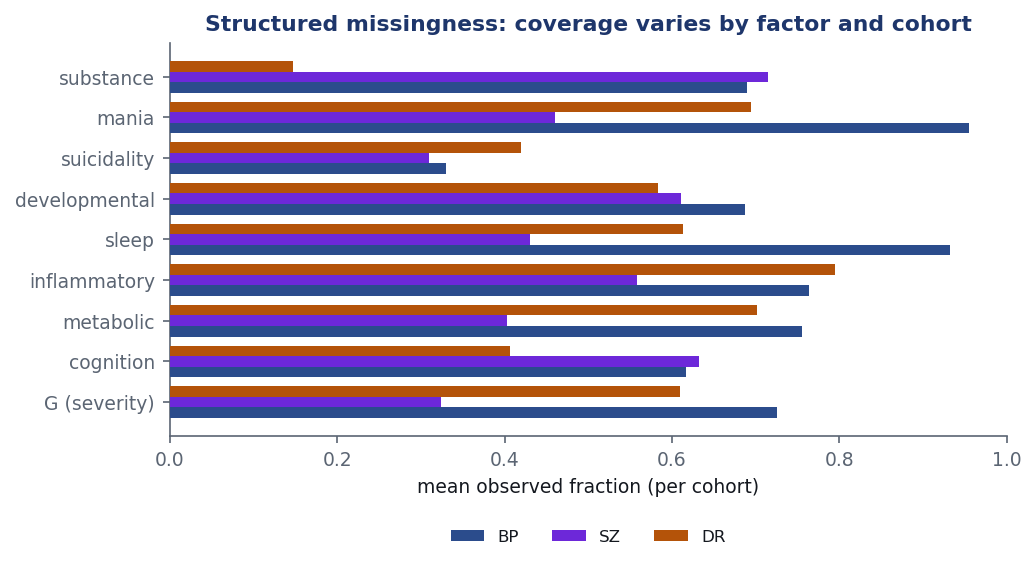
\includegraphics[width=0.82\linewidth]{figures/fig_coverage.png}
\caption{Observed coverage is structured, not random: it varies by factor block and by cohort. Mania
self-report and the depression/anxiety windows are thin or absent in some cohorts; biology and sleep are
broadly covered. The observed-data likelihood turns this structure from a liability into information.}
\label{fig:coverage}
\end{figure}

\begin{caveatbox}
The DR cohort ($N=552$) is small and lacks several instruments (e.g.\ FAST, QIDS, MADRS). Factors whose anchors
are cohort-specific are tested for measurement invariance (Chapter~\ref{sec:validation}) and their per-patient
reliability is flagged by observed-indicator count, rather than assuming a uniform map across cohorts.
\end{caveatbox}
